\begin{problem}
  Let $\mathcal{A}$ be the 3-dimensional space of functions on
  $[-1,1]$ composed of two straight line segments joined at $x =
  0$. Calculate the element of $\mathcal{A}$ that minimizes
  \begin{equation}
    \label{eq:integral}
\int_{-1}^1 \lvert x^2 - p(x) \rvert \, \text{dx}, \quad p \in \mathcal{A}.
\end{equation}
\end{problem}


\begin{solution}
$\mathcal{A}$ is a Haar space as if a function in $\mathcal{A}$ has
more than 2 zeros it is identically zero. Which can be taken as the
definition of a Haar space.

We then note that the equation \ref{eq:integral} is the 1-norm and the
element in $\mathcal{A}$ we are searching for is the best $L_1$
approximation from $\mathcal{A}$ to $x^2$. Now we use our dear theorem
14.5 again, giving us the zeros of the error function. These are given
by equation~\ref{eq:zeros}.
\begin{equation}
  \label{eq:zeros}
\zeta_k = \cos{\left (\pi \left(- \frac{k}{4} + \frac{3}{4}\right)
  \right )}
  \Leftrightarrow
  \begin{cases}
    \zeta_0 = - \frac{\sqrt{2}}{2} \\
    \zeta_1 = 0 \\
    \zeta_2 = \frac{\sqrt{2}}{2} \\
  \end{cases}
\end{equation}

By demanding that the error function have these three zeros we get a
candidate for a best approximation $p^*$ in
equation~\ref{eq:pstar}.

\begin{equation}
  \label{eq:pstar}
  p^*(x)  = 
  \begin{cases}
    - \frac{\sqrt{2} x}{2} & \text{for}\: x < 0 \\
    \frac{\sqrt{2} x }{2} & \text{for}\: x \geq 0    
  \end{cases}
\end{equation}

\begin{equation}
  \label{eq:task_4:error}
  x^2 - p^*(x)  = 
  \begin{cases}
    x^{2} + \frac{\sqrt{2} x}{2} & \text{for}\: x < 0 \\
    x^{2} - \frac{\sqrt{2} x}{2} & \text{for}\: x \geq 0
  \end{cases}
\end{equation}

The only thing remaining is to check that the criteria of there being
exactly 3 zeros in the error function is meet. In this case solving
for all the zeros becomes solving a piece wise defined second order
polynomial which is indeed possible. One need not however solve the
equations explicitly. Instead we note that second order polynomials
can have at most 2 zeros and both parts of the error in
equation~\ref{eq:task_4:error} are second order polynomials with one
root in common ($x = 0$). We thus conclude that the error function has
at most 3 zeros and we know by construction that it has 3
zeros. Therefore we know it has {\bf exactly } three zeros. Thus we
have found an element of $\mathcal{A}$ that minimizes
equation~\ref{eq:integral}. Further as $\mathcal{A}$ is an Haar space
the best approximation is unique. 

    
% \begin{figure}[!ht]
%   \centering
%   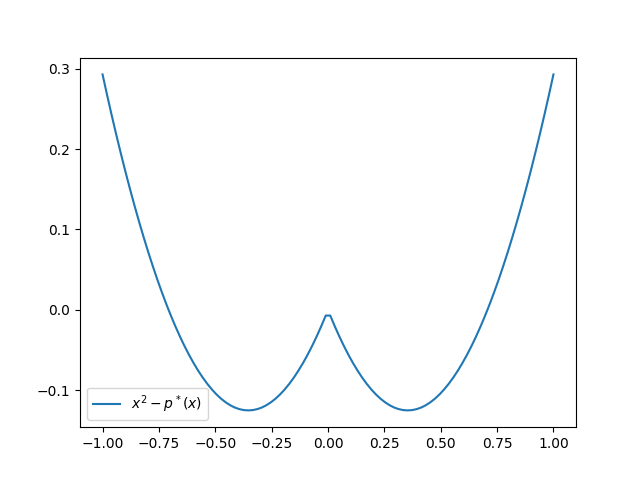
\includegraphics[scale = 0.5]{task_4_error.png}
%   \caption{Plot of $f - p^*$. Note that there is exactly 3 zeros!.}
%   \label{fig:task_3:error}
% \end{figure}

\end{solution}


%%% Local Variables:
%%% mode: latex
%%% TeX-master: "report"
%%% End:
